\section{Class diagram}
\label{rear:classdiagram}

Let us have a look at \framework{} class diagram, 
showed in figure \ref{fig:class_diagram}.

\ifthenelse{\isodd{\thepage}}{
\begin{figure}[!h]
  \begin{center}
    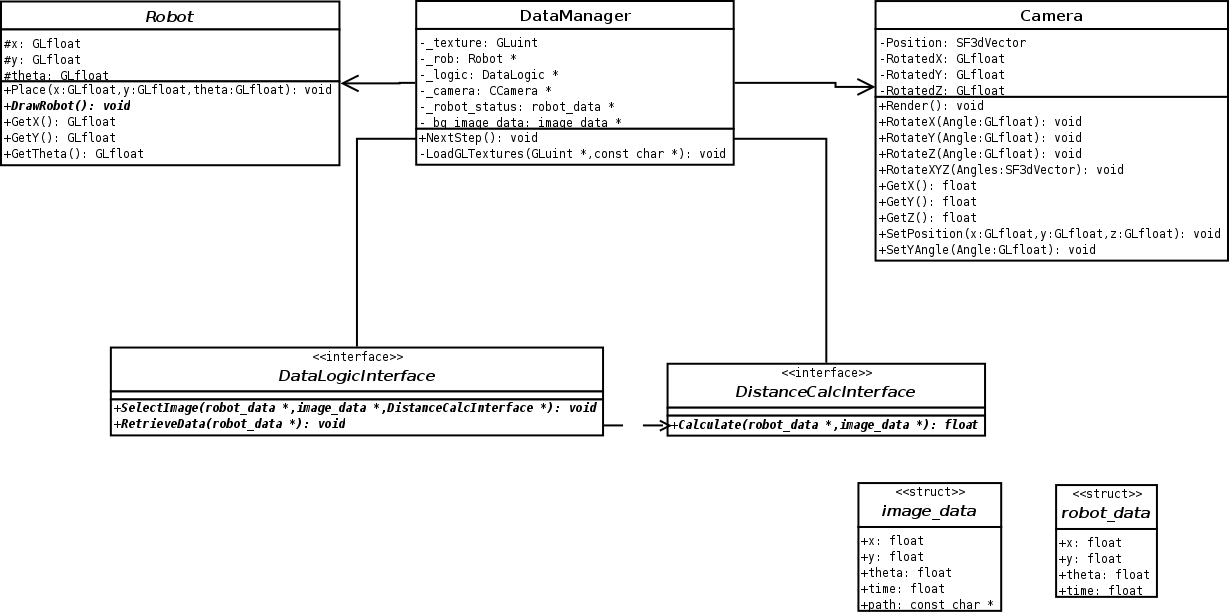
\includegraphics[width=\textheight, angle=90]{img/rear_class_diagram.png}
    \caption{\framework{} class diagram}
    \label{fig:class_diagram}
  \end{center}
\end{figure}
}
{
\begin{figure}[!h]
  \begin{center}
    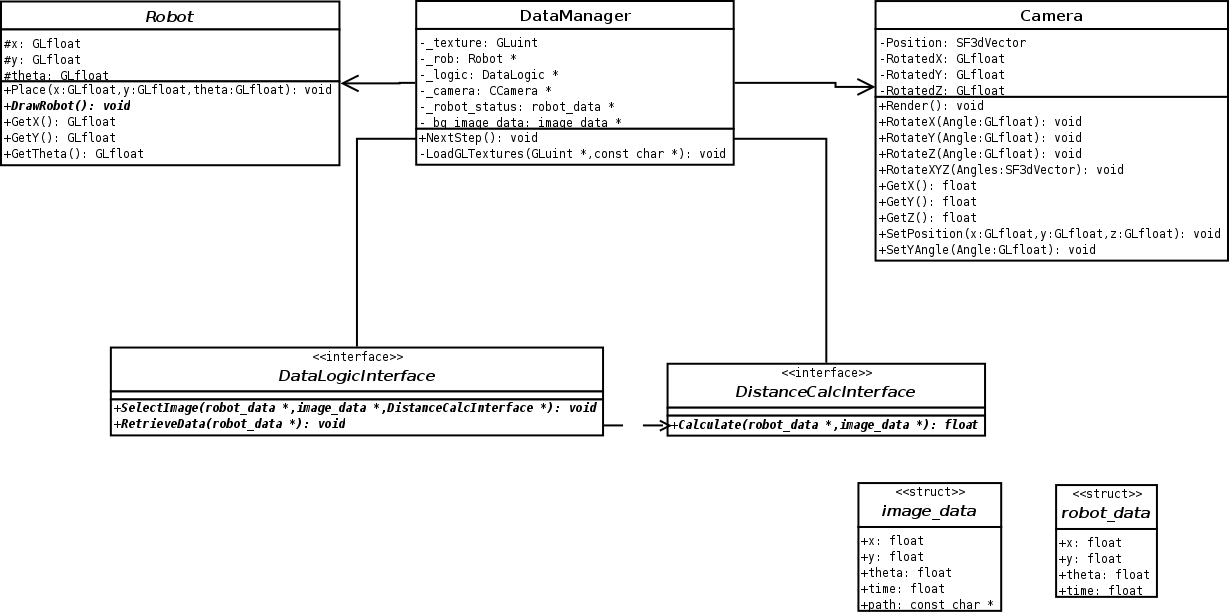
\includegraphics[width=\textheight, angle=270]{img/rear_class_diagram.png}
    \caption{\framework{} class diagram}
    \label{fig:class_diagram}
  \end{center}
\end{figure}
}

Two of the components needed by \framework{}, the robot 
model and the camera, are mapped on two dedicated classes, 
\texttt{Robot} and \texttt{Camera}, respectively.
\\
The former is an \textit{abstract class}, serving as a storage 
for the current position and orientation of the actual
robot and declare a pure virtual method in which subclasses 
must include all of the procedure to draw the OpenGL model 
of the robot itself.
\\
The latter is instead a \textit{helper class}, since 
exists no actual camera within the OpenGL space. The camera 
model is just an abstraction used to give a more intuitive
way to set the portion of space the user is looking at.
In fact, the \texttt{Camera} class provides methods to 
set the user's point-of-view within the OpenGL space (we
refer to section \ref{rear:classes:cameraclass}).
\\
In the middle, between \texttt{Robot} and \texttt{Camera},
there is the \texttt{DataManager} class. It is intended to be 
the core of every \framework{} based application, since it 
internally implements the loop showed in figure 
\ref{fig:overall_diagram}.
It acts as a \textit{mediator} among all of the other classes, 
in that it manages their interaction and, hence, reduces 
coupling between them.
\\
The diagram also features two interfaces that have to be implemented 
by programmers who want to create their own concrete exocentric 
vision system: \texttt{IDataLogic} and 
\texttt{IImageSelector}.
\\
\texttt{IDataLogic} decouples the application 
core, that is the \texttt{DataManager}, from the data source.
This way, \texttt{DataManager} code can be totally unaware of 
the technology used to retrieve data from the robot - e.g. 
sockets, web services, etc.
\\
\texttt{IImageSelector}, instead, defines the interface 
of the component which implements the image selection algorithm.
In this case, the use of an interface leaves programmers 
able to change, and even to implement new image 
selection algorithms without having to worry about
changing other classes.
\\
Finally, the class diagram presents two structures, 
\texttt{image\_data} and \texttt{robot\_data}, whose 
declarations are reported in listing \ref{code:data}.
\\
The former is used to store all the metadata 
relative to a specific snapshot - i.e. the position 
and the orientation of the camera when it was taken, 
a timestamp and an array of chars that can be used by 
programmers who would like to add other data - e.g. 
a code or a sequence number. More often this field is
exploited to store the file system path where the
image is stored.
\\
\texttt{robot\_data} structure is similar to the former,
it is meant to be 
used by \texttt{DataManager} to exchange information
about the current robot position and orientation with 
lower-level objects, in a compact way.
\\
\begin{lstlisting}[caption={\framework{} data structures}, label={code:data}]
struct image_data {
  float x;
  float y;
  float theta;
  float time;
  char path[100];
};

struct robot_data {
  float x;
  float y;
  float theta;
  float time;
};
\end{lstlisting}

In the following of this section, we will have a look 
\textit{under the hood} of the classes and interfaces 
we have just introduced.
We will see how \framework{} functionalities are 
mapped onto them and, then, how to correctly subclass/use
them in order to build a concrete exocentric vision system
(chapter \ref{concr}).
